\seminar{30}


\subsection*{Téma}
Hra SET

\teachernote{
\subsection*{Ciele}
Zoznámenie sa s hrou SET a riešenie jednoduchších aj zložitejších úloh využívajúcich vlastnosti herných kartičiek.



\subsubsection*{Úvodný komentár}

Seminár má trochu odlišnú štruktúru, než na akú boli študenti v seminároch doteraz navyknutí, no nepovažujeme to za žiadny problém. Taktiež je tento a nasledujúci seminár zaradený ako odľahčenie po tom, čo matematická olympiáda kategórie C vyvrcholila v uplynulom týždni.

\subsection*{Priebeh seminára}

\subsubsection*{Kartičky v hre SET}

Hra SET je kartovou hrou pre dvoch a viac hráčov. Každá kartička zobrazuje sadu symbolov, ktorá má 4 charakteristiky, pričom každá sa vyskytuje v~troch variantoch:
\begin{enumerate}
\item \textit{farba}: červená, modrá, zelená;
\item  \textit{tvar}: obdĺžnik, ovál, trojuholník;
\item \textit{výplň}: plná, polovičná, úplne biela;
\item \textit{počet symbolov}: jeden, dva, tri.
\end{enumerate}

\begin{tcolorbox}[breakable,notitle,boxrule=0pt,colback=light-gray,colframe=light-gray]\ul{30.1} Koľko kariet obsahuje hrací balíček? \end{tcolorbox}
\rie Keďže každá zo 4 charakteristík sa môže vyskytnúť v~troch rôznych variantoch, v~balíčku je celkom $3^4=81$ rôznych kartičiek. \\
\\
\kom Na seminár je vhodné mať kartičky nastrihané a zalaminované, aby sa s~nimi študentom lepšie manipulovalo. Príklad kartičiek je v prílohe.

\subsubsection*{Zoznámenie sa s~hrou SET}
SET je trojica kartičiek, pre ktorú platí: každá z~charakteristík je buď pre všetky tri kartičky rovnaká, alebo je na každej kartičke odlišná. Ak sa napríklad pozrieme na charakteristiku \textit{tvar}, tak sú na všetkých troch kartičkách buď len samé ovály (alebo len samé obdĺžniky, alebo len samé trojuholníky), alebo sú na jednej kartičke ovály, na druhej obdĺžniky a na tretej trojuholníky. Podobne pre ďalšie charakteristiky. \\
\\ \vspace{10pt}
\noindent
\begin{minipage}{.4\textwidth}
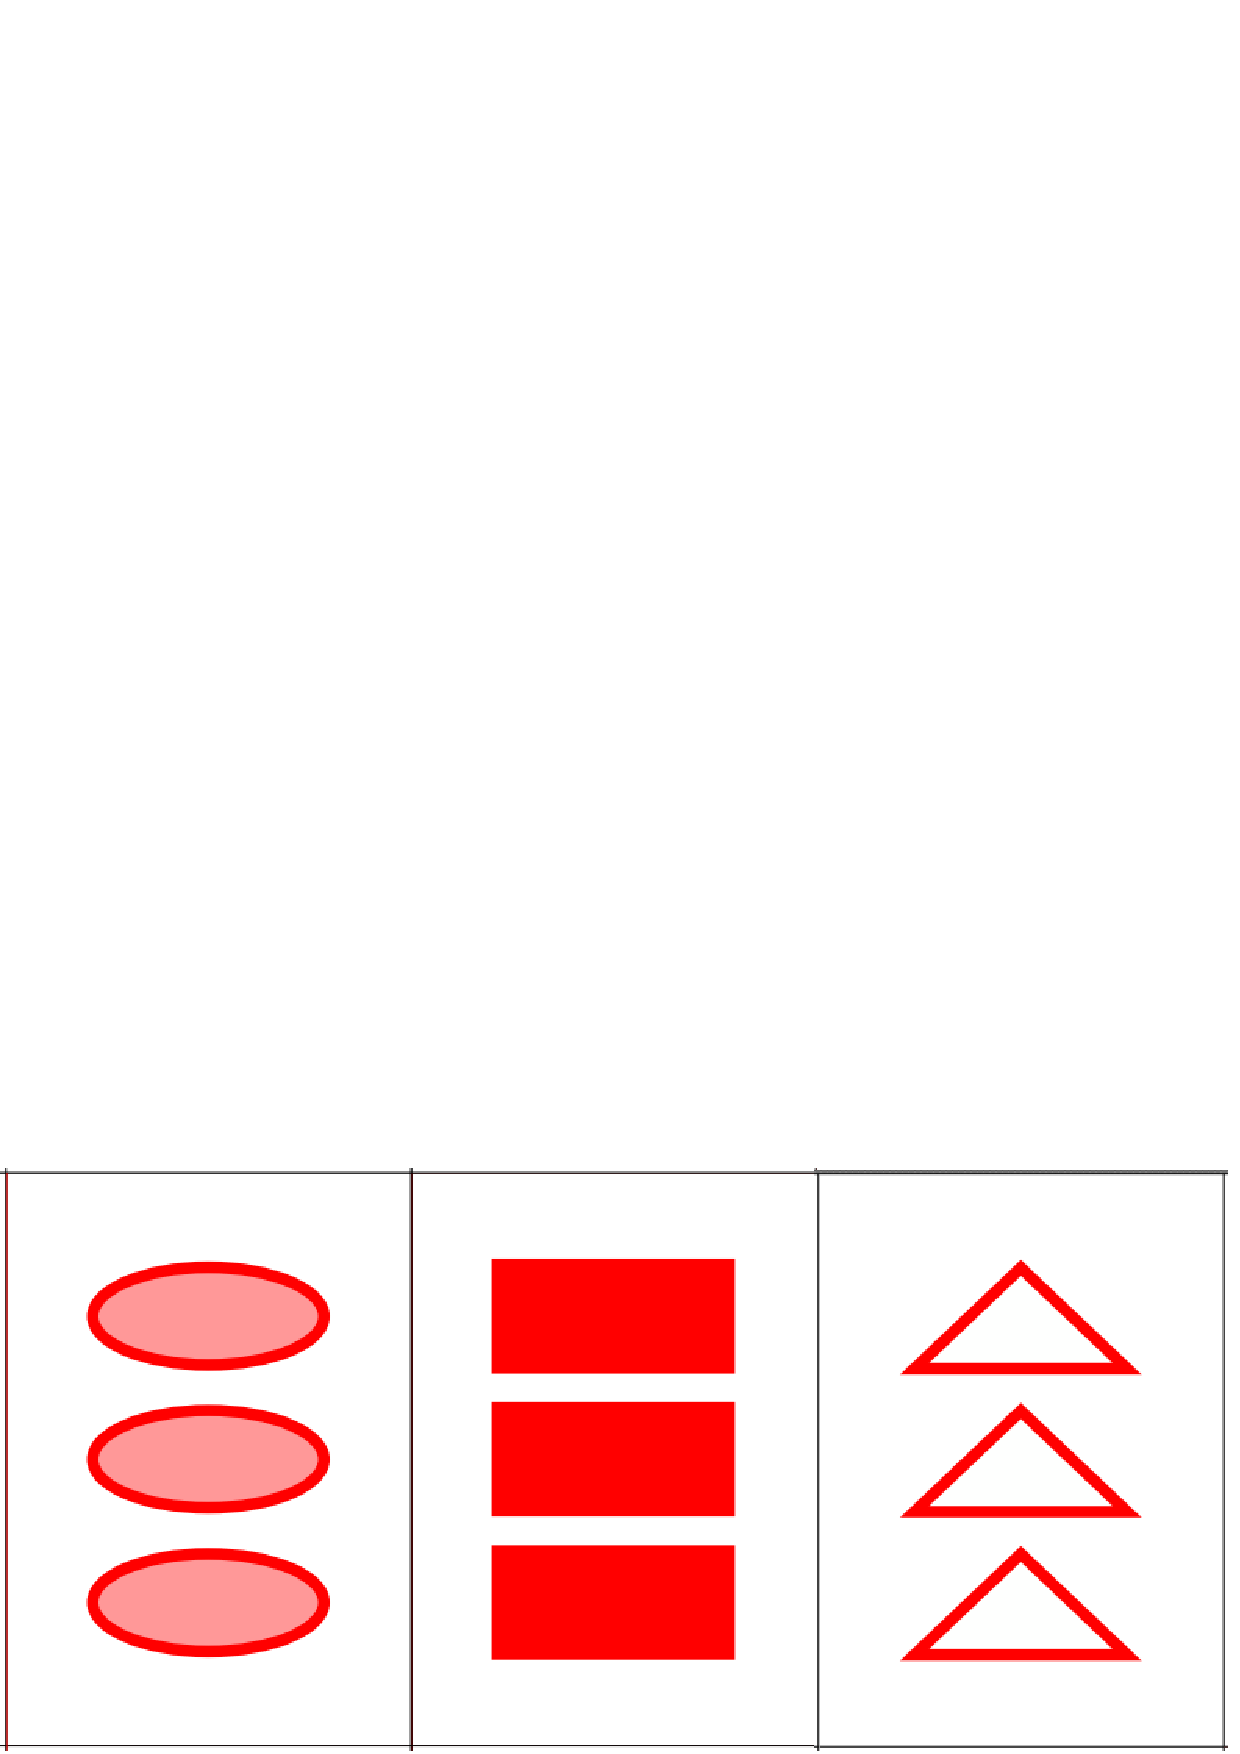
\includegraphics[width=0.8\textwidth]{images/set_ano.png}\\
Táto trojica kartičiek tvorí SET: farba je rovnaká, tvar je na každej kartičke iný, podobne výplň a všetky majú rovnaký počet symbolov. \\
\\

\end{minipage}% This must go next to `\end{minipage}`
\hspace{20pt}\begin{minipage}{.4\textwidth}
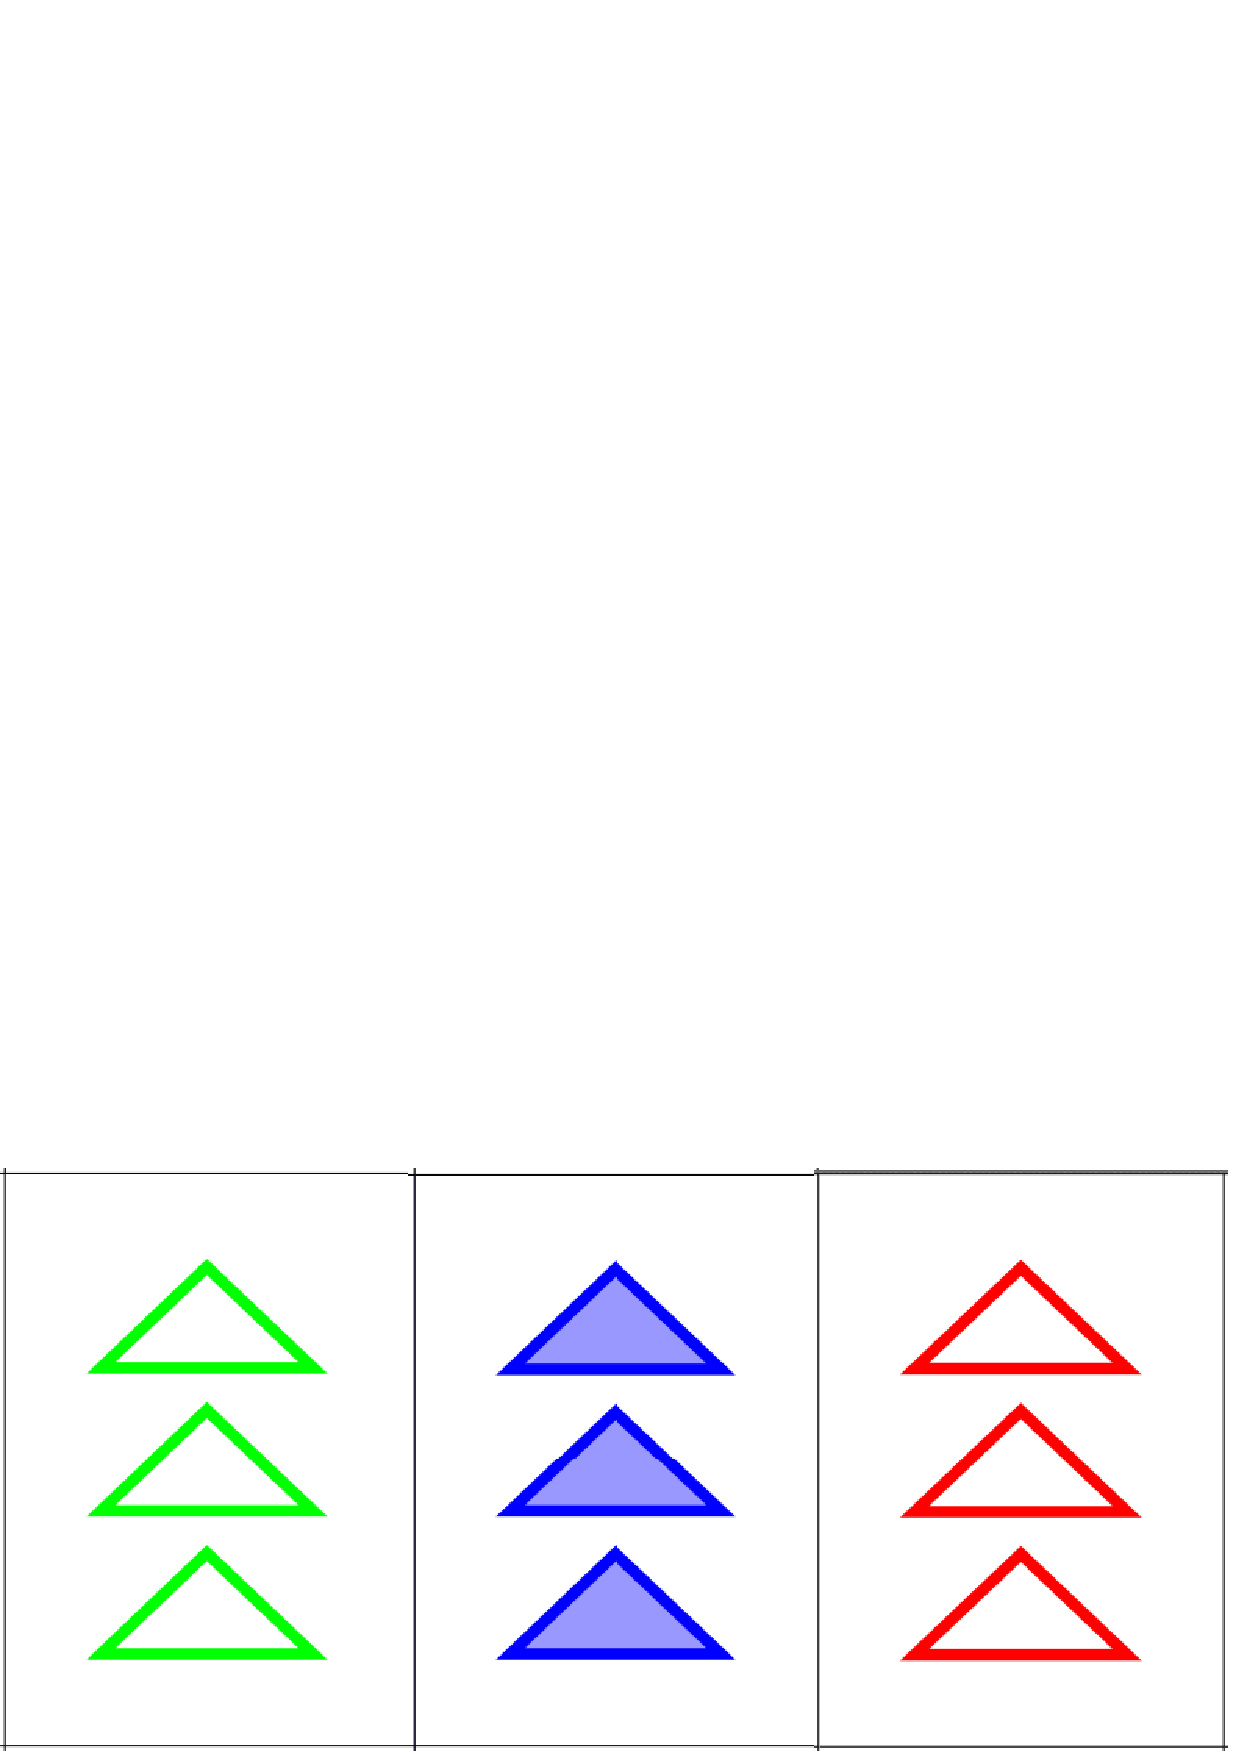
\includegraphics[width=0.8\textwidth]{images/set_nie.png}\\
Táto trojica nie je SET. Síce majú všetky tri kartičky rovnaký počet symbolov, symboly sú rovnakého tvaru a každá kartička je inej farby, výplň na dvoch kartičkách je prázdna zatiaľ čo tretia je vyplnená polovične.
\end{minipage}

Po zamiešaní sa z~balíčka vyloží na stôl 12 kartičiek. Hráči medzi nimi hľadajú SETy. Ak sa to niekomu podarí, vykríkne \uv{SET!} a ukáže ho spoluhráčom. Ak je SET správny, hráč si ho vezme zo stola, namiesto neho sa vyložia nové tri kartičky a pokračuje sa v~hre. V~prípade, že sú hráči presvedčení, že sa medzi vyloženými kartičkami žiadny SET nenachádza, doložia na stôl ďalšie tri kartičky. Hra končí v~momente, kedy hráči vyčerpajú všetky kartičky. Cieľom hry je, samozrejme, pozbierať čo najviac SETov. Hra sa dá hrať v~takmer ľubovoľne veľkej skupine, z~praktických dôvodov sa najviac osvedčili trojice a štvorice.\\
\\
\kom Predtým, než sa pustíme do hrania, je vhodné so študentmi prejsť niekoľko trojíc kartičiek a pobaviť sa o~tom, ktoré trojice SETmi sú, ktoré nie a prečo, prípadne premietnuť rozloženie 12 kartičiek a hľadať v~nich SETy spoločne. \\
\\
Po zahraní niekoľkých kôl sa so študentmi pobavíme o~tom, akým spôsobom SETy hľadali, ktoré SETy sú na nájdenie jednoduchšie, prípadne iné ďalšie zaujímavosti, ktoré počas hry vypozorovali. K~tejto diskusii sa môžeme vrátiť neskôr v~priebehu seminára, keď sa budeme zaoberať kategorizovaním rôznych typov SETov.

\subsubsection*{Úlohy o~balíčku kariet}
\begin{tcolorbox}[breakable,notitle,boxrule=0pt,colback=light-gray,colframe=light-gray]\ul{30.2} Ak vyberiem dve ľubovoľné kartičky z~balíčka, koľko kartičiek existuje takých, aby s~pôvodnými dvoma tvorili SET a prečo? \end{tcolorbox}

\rie Taká kartička je práve jedna, keďže charakteristiky prvých dvoch priamo určujú, aká variácia každej charakteristiky musí byť na poslednej kartičke (ak sa prvé dve kartičky v~charakteristike zhodujú, musí sa s~nimi zhodovať aj tretia, ak sú odlišné, aj tretia kartička sa musí odlišovať).\\
\\
\begin{tcolorbox}[breakable,notitle,boxrule=0pt,colback=light-gray,colframe=light-gray]\ul{30.3} Koľko rôznych SETov (kartičky sa v~rámci jednotlivých SETov môžu opakovať) sa nachádza v~celom balíčku?\end{tcolorbox}

\rie  Na vytvorenie SETu potrebujeme tri kartičky. Prvú z~nich môžem bez akéhokoľvek obmedzenia vybrať spomedzi všetkých 81 kartičiek, druhá kartička sa dá vybrať 80 spôsobmi a z~predchádzajúceho vieme, že tretia kartička tvoriaca SET s~už dvoma zvolenými je práve jedna. Keďže však nezáleží na poradí, v~ktorom sme kartičky vyberali, vydelíme počet možností $81\cdot80$ počtom všetkých možných usporiadaní troch kartičiek, teda $6$. Celkom dostávame $\frac{81\cdot80}{6}=1080$ rozličných SETov.\\
\\
\begin{tcolorbox}[breakable,notitle,boxrule=0pt,colback=light-gray,colframe=light-gray]\ul{30.4} Z~balíčka vyberieme jednu kartičku. Koľkých rôznych SETov môže byť táto kartička súčasťou?\end{tcolorbox}
\rie  Z~predchádzajúceho plynie, že zvyšných 80 kartičiek v~balíčku vieme rozdeliť na 40 neprelínajúcich sa dvojíc, pričom každá táto dvojica bude tvoriť s~pôvodnou kartičkou SET.\\
\\
\kom Menej zdatným študentom môže s~pochopením vysvetlenia pomôcť vyložiť si na stôl konkrétne dvojice -- teda hľadať konkrétne SETy, ktorých je vybraná kartička súčasťou. \\
\\
\begin{tcolorbox}[breakable,notitle,boxrule=0pt,colback=light-gray,colframe=light-gray]\ul{30.5} Ako je možné ukázať, že v~danom rozložení kartičiek na stole sa nenachádza žiadny SET?\end{tcolorbox}
\rie  K~tomuto problému je možné pristupovať rôznymi spôsobmi, no všetky spája potreba skontrolovať všetky možné kombinácie a vylúčiť prítomnosť SETu. Zaujímavé je pozorovať, akú stratégiu študenti zvolia (v~porovnaní s~tým, ako postupovali pri hraní hry).  Nástavbou na túto úlohu môže byť otázka, ako dané rozloženie 12 kartičiek  skontrolovať čo najefektívnejšie.\\
\\

\begin{tcolorbox}[breakable,notitle,boxrule=0pt,colback=light-gray,colframe=light-gray]\ul{30.6} Je možné SETy nejako kategorizovať? Ako? Koľko SETov v~jednotlivých kategóriách je možné vytvoriť? Vieme správnosť našich výpočtov overiť pomocou nejakých predchádzajúcich úvah?\end{tcolorbox}
\rie Táto úloha sa dá opäť uchopiť mnohými spôsobmi. Jedným z~nich môže byť roztriedenie SETov pomocou počtu charakteristík, ktoré majú kartičky spoločné. Každé rozdelenie, ktoré žiaci vymyslia, by ich však v~konečnom dôsledku malo priviesť k~rovnakému počtu SETov ako v~úlohe 2.\\
\\
\textbf{Záverečný komentár.} Hra SET je pre študentov (a nielen nich) veľmi atraktívna a majú tendencie sa odhodlane púšťať aj do predkladaných problémov. Stretnutie je tak príjemnou zmenou tempa a obsahu doterajšieho priebehu seminára

\subsubsection*{Doplňujúce zdroje a materiály}

Výborným sprievodcom plným zaujímavých úloh spolu s komentovanými študentskými riešeniami je možné nájsť na \cite{SET}.


}

